\documentclass[10pt,a4paper, margin=1in]{article}
\usepackage{fullpage}
\usepackage{amsfonts, amsmath, pifont}
\usepackage{amsthm}
\usepackage{graphicx}

\usepackage[utf8]{inputenc}

\usepackage{float}
\usepackage{tkz-euclide}
\usepackage{tikz}
\usepackage{pgfplots}
\pgfplotsset{compat=1.13}

\usepackage{geometry}
 \geometry{
 a4paper,
 total={210mm,297mm},
 left=10mm,
 right=10mm,
 top=10mm,
 bottom=10mm,
 }
 \author{
  Yesilyurt, Yavuz Selim\\
  \texttt{e2259166@ceng.metu.edu.tr}
  \and
   Simsek, Halit\\
  \texttt{e2099760@ceng.metu.edu.tr}
}
\title{CENG 384 - Signals and Systems for Computer Engineers \\
Spring 2018-2019 \\
Written Assignment 1}

\begin{filecontents}{q3.dat}
  n  xn
 -8  0
 -7  3
 -6  0  
 -5  0
 -4 -4
 -3  0
 -2  2
 -1 -1
  0 -1
  1  0
  2  0
  3  3
\end{filecontents}

\begin{filecontents}{q5_1.dat}
  n  xn
 -8  0
 -7  1.5
 -6  0  
 -5  0
 -4 -2
 -3  0
 -2  1
 -1 -0.5
  0  0
  1 -0.5
  2  1
  3  0
  4 -2
  5  0
  6  0
  7  1.5
  8  0
\end{filecontents}

\begin{filecontents}{q5_2.dat}
  n  xn
 -8  0
 -7 -1.5
 -6  0  
 -5  0
 -4  2
 -3  0
 -2 -1
 -1  0.5
  0  0
  1 -0.5
  2  1
  3  0
  4 -2
  5  0
  6  0
  7  1.5
  8  0
\end{filecontents}

\begin{document}
\maketitle



\noindent\rule{19cm}{1.2pt}

\begin{enumerate}

\item 
    \begin{enumerate}
    \item
    Given $z = x + yj$ and $3z + 4 = 2j - \Bar{z}$, finding $\Bar{z}$ which is conjugate of $z$: \\
    $\Bar{z} = x - yj$ \\
    Applying the $z$ and $\Bar{z}$ to the given equation: \\
    $3(x + yj) + 4 = 2j - (x - yj)$ \\
    $4x + 2yj = -4 + 2j$ \\
    $x = -1$ \\
    $y = 1$ \\
    Putting the values $x$ and $y$ in the $z$ \\
    $z = -1 + j$ \\
    $|z| = \sqrt{(-1)^2 + (1)^2} = \sqrt{2}$ \\
    $|z|^2 = 2$ \\
    
    \begin{tikzpicture}
        \begin{scope}[thick,font=\scriptsize]
        % Axes:
        % Are simply drawn using line with the `->` option to make them arrows:
        % The main labels of the axes can be places using `node`s:
        \draw [->] (-5,0) -- (5,0) node [above left]  {$\Re\{z\}$};
        \draw [->] (0,-5) -- (0,5) node [below right] {$\Im\{z\}$};
    
        % Axes labels:
        % Are drawn using small lines and labeled with `node`s. The placement can be set using options
        \iffalse% Single
        % If you only want a single label per axis side:
        \draw (1,-3pt) -- (1,3pt)   node [above] {$1$};
        \draw (-1,-3pt) -- (-1,3pt) node [above] {$-1$};
        \draw (-3pt,1) -- (3pt,1)   node [right] {$i$};
        \draw (-3pt,-1) -- (3pt,-1) node [right] {$-i$};
        \else% Multiple
        % If you want labels at every unit step:
        \foreach \n in {-4,...,-1,1,2,...,4}{%
            \draw (\n,-3pt) -- (\n,3pt)   node [above] {$\n$};
            \draw (-3pt,\n) -- (3pt,\n)   node [right] {$\n i$};
        }
        \fi
        \end{scope}
        % The circle is drawn with `(x,y) circle (radius)`
        % You can draw the outer border and fill the inner area differently.
        % Here I use gray, semitransparent filling to not cover the axes below the circle
        % \path [draw=black] (0, 0) circle (1.414213562);
        % Place the equation into the circle:
        \draw [blue, line width=0.8] (0, 0) -- (-1, 1) node [left, blue] {$z = -1 + j$};
    \end{tikzpicture}
    
    \item
    Given $z = re^{j \theta }$: \\
    $z^3 = r^3e^{j3 \theta} = 64j$ \\
    This equation gives us: \\
    $r = 4$, \\
    $e^{j3 \theta } = j$ \\
    Remembering equation ($e^{j \theta } = \cos{ \theta } + j \sin{ \theta })$: \\
    $e^{j3 \theta } = j = \cos{( \frac{ \pi }{2})} + j \sin{(\frac{ \pi }{2})}$ \\
    Therefore: \\
    $3 \theta = \frac{ \pi }{2}$ \\
    $ \theta = \frac{ \pi }{6}$ \\
    $z$ in polar form: \\
    $z = 4( \cos{( \frac{ \pi }{6}}) + j \sin{( \frac{ \pi }{6})})$ \\
    $z = 4e^{(j\frac{ \pi }{6} + \frac{2 \pi }{3} k)}$ where k=1,2,3,... \\
    \item
    Multiplying both numerator and denominator of given $z$ with $(1 - j)$: \\
    $z = \frac{(1 - j)^2(1 + \sqrt{3}j)}{(1 + j)(1 - j)} = \frac{(1 - j)^2(1 + \sqrt{3}j)}{2} = \frac{(-2j)(1 + \sqrt{3}j)}{2} = (-j)(1 + \sqrt{3}j) = \sqrt{3} - j$ \\
    \\
    Finding magnitude $r$ and angle $ \theta $ of $z$: \\
    $r = \sqrt{( \sqrt{3})^2 + (1)^2} = 2$ \\
    $ \theta = 2 \pi - \arctan{( \frac{1}{\sqrt{3}} )} = \frac{11 \pi }{6}$ \\
    \item
    Given $z$, $-j$ can be rewritten as: \\
    $-j = \cos{( \frac{3 \pi }{2})} + j \sin{( \frac{3 \pi }{2})} = e^{j \frac{3 \pi }{2}}$ \\
    \\
    Therefore $z$ can be rewritten as: \\
    $z = e^{j \frac{3 \pi }{2}} e^{j \frac{ \pi }{2}} = e^{j 2 \pi }$ \\
    \end{enumerate}


\item 
Below is the signal for $y(t) = x(\frac{1}{2}t + 1)$
\begin{figure}[H]
    \centering
        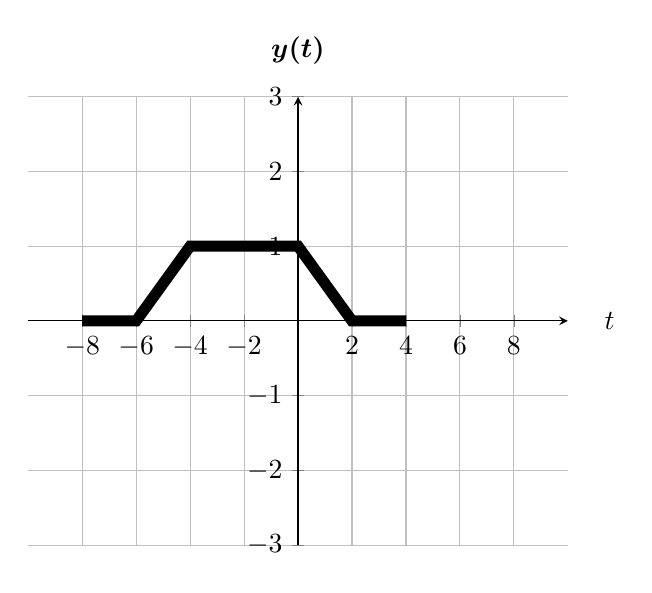
\begin{tikzpicture}[scale=1.0]
           \begin{axis}[
          axis lines=middle,
          xlabel={$t$},
          ylabel={$\boldsymbol{y(t)}$},
          xtick={-8, -6, -4, -2, ..., 8},
          ytick={-3, -2, -1, ..., 3},
          ymin=-3, ymax=3,
          xmin=-10, xmax=10,
          every axis x label/.style={at={(ticklabel* cs:1.05)}, anchor=west,},
          every axis y label/.style={at={(ticklabel* cs:1.05)}, anchor=south,},
          grid,
        ]
           \path[draw,line width=4pt] (-8,0) -- (-6,0) -- (-4,1) -- (0,1) -- (2,0) -- (4,0);
           \end{axis}
        \end{tikzpicture}
        \caption{$t$ vs. $y(t)$.}
        \label{fig:q2}
    \end{figure}


\item   
\begin{enumerate}
    \item 
    Below is the signal for $x[-n] + x[2n + 1]$
\begin{figure}[H]
    \centering
    \begin{tikzpicture}[scale=1.0] 
      \begin{axis}[
          axis lines=middle,
          xlabel={$n$},
          ylabel={$\boldsymbol{x[-n]+x[2n+1]}$},
          xtick={ -9, -8, ..., 4},
          ytick={-4, -3, -2, -1, ..., 4},
          ymin=-4, ymax=4,
          xmin=-9, xmax=4,
          every axis x label/.style={at={(ticklabel* cs:1.05)}, anchor=west,},
          every axis y label/.style={at={(ticklabel* cs:1.05)}, anchor=south,},
          grid,
        ]
        \addplot [ycomb, black, thick, mark=*] table [x={n}, y={xn}] {q3.dat};
      \end{axis}
    \end{tikzpicture}
    \caption{$n$ vs. $x[-n]+x[2n+1]$.}
    \label{fig:q3}
\end{figure}
    
    \item 
    $x[-n] + x[2n+1]$ in terms of the unit impulse function is as follows:\\
    
    $3\delta(n+7)-4\delta(n+4)+2\delta(n+2)-\delta(n+1)-\delta(n)+3\delta(n-3)$ \\
    \end{enumerate}

\newpage

\item 
    \begin{enumerate}
    \item To check if any signal is periodic or aperiodic we have the following: \\ $x(t)$ is periodic if $\exists T$ such that $x(t) = x(t+T)$ and $x(n)$ is periodic if $\exists N \epsilon I$ such that $x(n) = x(n+N)$. \\
     In continious case, we can find fundamental period with $T=\frac{2\pi}{\omega}$ and in discrete case, we can find fundamental period with $N=\frac{2\pi}{\Omega}$. For parts a,b,c and d these information will be used. \\
We have: \\
\begin{center}
$x[n] = 3cos[\frac{13\pi}{10}n] + 5sin[\frac{7\pi}{3}n - \frac{2\pi}{3}]$ 
\end{center}
This is a discrete signal, according to information mentioned above, fundamental period for $3cos[\frac{13\pi}{10}n]$ (Since this is a discrete signal we need an integer $m$ to make $N$ integer):
\begin{align*}
N_1&=\frac{2\pi}{\Omega}m \\
N_1&=\frac{2\pi}{\frac{13\pi}{10}}m \\
N_1&=\frac{20}{13}m \ \ \ \ \ \ m = 13 \\
N_1&=20
\end{align*}
Fundamental period for $5sin[\frac{7\pi}{3}n - \frac{2\pi}{3}]$ (Since this is a discrete signal we need an integer $m$ to make $N$ integer):
\begin{align*}
N_2&=\frac{2\pi}{\Omega}m \\
N_2&=\frac{2\pi}{\frac{7\pi}{3}}m \\
N_2&=\frac{6}{7}m \ \ \ \ \ \ m = 7 \\
N_2&=6
\end{align*}
To be able to find fundamental period for $x[n]$ we need to find $lcm(N_1,N_2)$:
\begin{align*}
N &= lcm(N_1,N_2) \\
N &= lcm(20,6) \\
N&=60
\end{align*}
60 is the fundamental period of $x[n]$.\\

    \item We have: 
\begin{center}
$x[n] = 5sin[3n - \frac{\pi}{4}]$ 
\end{center}
This is also a discrete signal, according to information mentioned in part a, fundamental period can be found as:
\begin{align*}
N&=\frac{2\pi}{\Omega}m \\
N&=\frac{2\pi}{3}m
\end{align*}
There does not exist any integer $m$ which can make $N=\frac{2\pi}{3}m$ integer, so we can safely say $x[n]$ is an aperiodic signal. \\
    
    \item We have: 
\begin{center}
$x(t) = 2cos(3\pi t - \frac{2\pi}{5})$ 
\end{center}
This is a continious signal, according to information mentioned in part a, fundamental period can be found as:
\begin{align*}
T&=\frac{2\pi}{\omega} \\
T&=\frac{2\pi}{3\pi} \\
T&=\frac{2}{3}
\end{align*}
$\frac{2}{3}$ is the fundamental period of $x(t)$.\\

\newpage

    \item We have: 
\begin{center}
$x(t) = -je^{j5t}$ 
\end{center}
This is also a continious signal, according to information mentioned in part a, fundamental period can be found as:
\begin{align*}
T&=\frac{2\pi}{\omega} \\
T&=\frac{2\pi}{5}
\end{align*}
$\frac{2\pi}{5}$ is the fundamental period of $x(t)$.\\

    \end{enumerate}

\item Let's first check whether the signal is even or odd. We see that $x[n]$ is neither even nor odd, since it does not have symmetry neither across $y$-axis nor across origin. To find even and odd decompositions of $x[n]$, we have:
\begin{align*}
x[n]&=\text{Ev\{x[n]\}} + \text{Odd\{x[n]\}} \\
x[n]&=\frac{1}{2}\{x[n]-x[-n]\} + \frac{1}{2}\{x[n]+x[-n]\}
\end{align*}
So $\text{Ev\{x[n]\}}$ can be drawn as: \\
\begin{figure}[H]
    \centering
    \begin{tikzpicture}[scale=1.0] 
      \begin{axis}[
          axis lines=middle,
          xlabel={$n$},
          ylabel={$\boldsymbol{\frac{1}{2}\{x[n]+x[-n]\}}$},
          xtick={ -9, -8, ..., 9},
          ytick={-2, -1.5, -1, -0.5, ..., 2},
          ymin=-2, ymax=2,
          xmin=-9, xmax=9,
          every axis x label/.style={at={(ticklabel* cs:1.05)}, anchor=west,},
          every axis y label/.style={at={(ticklabel* cs:1.05)}, anchor=south,},
          grid,
        ]
        \addplot [ycomb, black, thick, mark=*] table [x={n}, y={xn}] {q5_1.dat};
      \end{axis}
    \end{tikzpicture}
    \caption{$n$ vs. $\frac{1}{2}\{x[n]+x[-n]\}$.}
    \label{fig:q4}
\end{figure}
and $\text{Odd\{x[n]\}}$ can be drawn as: \\
\begin{figure}[H]
    \centering
    \begin{tikzpicture}[scale=1.0] 
      \begin{axis}[
          axis lines=middle,
          xlabel={$n$},
          ylabel={$\boldsymbol{\frac{1}{2}\{x[n-x[-n]\}}$},
          xtick={ -9, -8, ..., 9},
          ytick={-2, -1.5, -1, -0.5, ..., 2},
          ymin=-2, ymax=2,
          xmin=-9, xmax=9,
          every axis x label/.style={at={(ticklabel* cs:1.05)}, anchor=west,},
          every axis y label/.style={at={(ticklabel* cs:1.05)}, anchor=south,},
          grid,
        ]
        \addplot [ycomb, black, thick, mark=*] table [x={n}, y={xn}] {q5_2.dat};
      \end{axis}
    \end{tikzpicture}
    \caption{$n$ vs. $\frac{1}{2}\{x[n]-x[-n]\}$.}
    \label{fig:q5}
\end{figure}

\newpage

\item 
    \begin{enumerate}
    \item 
        \begin{enumerate}
        \item System needs memory since it needs to remember both past and future inputs for some of the outputs.
        \item The system is stable since its amplitude is bounded by a constant value and does not vary due to input.
        \item The System does \textit{not} depend on only past and present inputs, it has some future inputs too, so this system is not causal.
        \item For system to be linear, it needs to hold superposition property. So we need to check if this system holds superposition property. Let $x_1$ and $x_2$ be two input signals:
            \begin{align*}
            y_1(t) & =x_1(2t-3) \\
            y_2(t) & =x_2(2t-3)
            \end{align*}
            When we add these up and multiply by some scalars $a_1$ and $a_2$, we will have a $y_3$ as:
            \begin{align*}
            y_3(t)&= a_1 \times y_1(t) + a_2 \times y_2(t) \\
                  &= a_1 \times x_1(2t-3)+ a_2 \times x_2(2t-3)
            \end{align*}
            and on the other hand when we first perform addition and multiplication then put the signal as input to the system we will have a $y_3^{'}$ such as:
            \begin{align*}
                x_3(t)&=a_1\times x_1(t) + a_2\times x_2(t) \\
                y_3^{'}(t)&=x_3(2t-3)\\
                &=a_1\times x_1(2t-3) + a_2\times x_2(2t-3)
            \end{align*}
            Since $y_3 = y_3'$ superposition property holds and system is linear.
        \item The system is invertible since:
        \begin{align*}
        x(t) &= h^{-1}(y(t)) \\
             &= y(\frac{t+3}{2})
        \end{align*}
        \item We will check time invariance as follows:
        \begin{center}
        Let $x_1(t) = x(t-t_0)$ \\
        We will have $y(t)=x_1(2t-3)$ \\
        So $y(t) = x(2t-t_0-3)$
        \end{center}
        On the other hand we have:
        \begin{align*}
        y^{'}(t) &= y(t-t_0)  \\
                 &= x(2(t-t_0)-3)\\
                 &= x(2t-2t_0-3)
        \end{align*}
        Since $y(t) \neq y^{'}(t)$ system is time variant. \\
        \end{enumerate}
    \item
        \begin{enumerate}
        \item System does not need memory since it does not need to remember neither past nor future inputs. So this system is memoryless.
        \item The system is not stable since its amplitude is not bounded and it varies due to input.
        \item Since, system depends on only the present outputs, so this system is causal.
        \item For system to be linear, it needs to hold superposition property. So we need to check if this system holds superposition property. Let $x_1$ and $x_2$ be two input signals:
            \begin{align*}
            y_1(t) & =t \times x_1(t) \\
            y_2(t) & =t \times x_2(t)
            \end{align*}
            When we add these up and multiply by some constants $a_1$ and $a_2$, we will have a $y_3$ as:
            \begin{align*}
            y_3(t)&= a_1 \times y_1(t) + a_2 \times y_2(t) \\
                  &= a_1 \times t \times x_1(t)+ a_2 \times t \times x_2(t)
            \end{align*}
            and on the other hand when we first perform addition and multiplication then put the signal as input to the system we will have a $y_3^{'}$ such as:
            \begin{align*}
                x_3(t)&=a_1\times x_1(t) + a_2\times x_2(t) \\
                y_3^{'}(t)&=t \times x_3(t)\\
                &=a_1\times t \times x_1(t) + a_2\times t \times x_2(t)
            \end{align*}
            Since $y_3 = y_3'$ superposition property holds and system is linear.
        \item The system is invertible since:
        \begin{align*}
        x(t) &= h^{-1}(y(t)) \\
             &= \frac{1}{t} \times y(t)
        \end{align*}
        \item We will check time invariance as follows:
        \begin{center}
        Let $x_1(t) = x(t-t_0)$ \\
        We will have $y(t)=t \times x_1(t)$ \\
        So $y(t) = t \times x(t - t_0)$
        \end{center}
        On the other hand we have:
        \begin{align*}
        y^{'}(t) &= y(t-t_0) \\
        &= (t - t_0) \times x(t-t_0)
        \end{align*}
        Since $y(t) \neq y^{'}(t)$ system is time variant. \\
        \end{enumerate}
    \item 
        \begin{enumerate}
        \item System needs memory since it needs to remember both past and future inputs for some of the outputs.
        \item The system is stable since its amplitude is bounded by a constant value and does not vary due to input.
        \item The System does \textit{not} depend on only past and present inputs, it has some future inputs too, so this system is not causal.
        \item For system to be linear, it needs to hold superposition property. So we need to check if this system holds superposition property. Let $x_1$ and $x_2$ be two input signals:
            \begin{align*}
            y_1[n] & =x_1[2n-3] \\
            y_2[n] & =x_2[2n-3]
            \end{align*}
            When we add these up and multiply by some constants $a_1$ and $a_2$, we will have a $y_3$ as:
            \begin{align*}
            y_3[n]&= a_1 \times y_1[n] + a_2 \times y_2[n] \\
                  &= a_1 \times x_1[2n-3]+ a_2 \times x_2[2n-3]
            \end{align*}
            and on the other hand when we first perform addition and multiplication then put the signal as input to the system we will have a $y_3^{'}$ such as:
            \begin{align*}
                x_3[n]&=a_1\times x_1[n] + a_2\times x_2[n] \\
                y_3^{'}[n]&=x_3[2n-3]\\
                &=a_1\times x_1[2n-3] + a_2\times x_2[2n-3]
            \end{align*}
            Since $y_3 = y_3'$ superposition property holds and system is linear.
        \item The system is invertible since:
        \begin{align*}
        x[n] &= h^{-1}(y[n]) \\
             &= y[\frac{n+3}{2}]
        \end{align*}
        \item We will check time invariance as follows:
        \begin{center}
        Let $x_1[n] = x[n-n_0]$ \\
        We will have $y[n]=x_1[2n-3]$ \\
        So $y[n] = x[2n-n_0-3]$
        \end{center}
        On the other hand we have: 
        \begin{align*}
        y^{'}[n] &= y[n-n_0]  \\
                 &= x[2(n-n_0)-3]\\
                 &= x[2n-2n_0-3]
        \end{align*}
        Since $y[n] \neq y^{'}[n]$ system is time variant. \\
        \end{enumerate}
    \item
    \begin{enumerate}
        \item
        System needs memory since its output depends on the sum of all its past values of input. 
        \item
        The system is not stable since its amplitude is not bounded and it varies due to input. More specifically, even though each individual signal that makes up the sum is stable, their sum makes $y[n]$ unbounded since it goes up to $\infty$ .
        \item
        The system depends on only the past inputs, so this system is causal.
        \item For system to be linear, it needs to hold superposition property. So we need to check if this system holds superposition property. Let $x_1$ and $x_2$ be two input signals:
            \begin{align*}
            y_1[n] & = \sum_{k=1}^{\infty} x_1[n - k] \\
            y_2[n] & = \sum_{k=1}^{\infty} x_2[n - k]
            \end{align*}
            When we add these up and multiply by some constants $a_1$ and $a_2$, we will have a $y_3$ as:
            \begin{align*}
            y_3[n] &= a_1 \times y_1[n] + a_2 \times y_2[n] \\
                   &= a_1 \times \sum_{k=1}^{\infty} x_1[n - k] + a_2 \times \sum_{k=1}^{\infty} x_2[n - k]
            \end{align*}
            and on the other hand when we first perform addition and multiplication then put the signal as input to the system we will have a $y_3^{'}$ such as:
            \begin{align*}
                x_3[n] &= a_1\times x_1[n] + a_2\times x_2[n] \\
                y_3^{'}[n] &= \sum_{k=1}^{\infty} x_3[n - k]\\
                &= a_1\times \sum_{k=1}^{\infty} x_1[n - k] + a_2 \times \sum_{k=1}^{\infty} x_2[n -k]
            \end{align*}
            Since $y_3 = y_3'$ superposition property holds and system is linear. \\
        \item The system is invertible since:
        \begin{align*}
        x[n] &= h^{-1}(y[n]) \\
             &= y[n + 1] - y[n] \\
             &= \{x[n] + x[n-1] + ...\} - \{x[n-1] + x[n-2] + ...\} 
        \end{align*}
        
        \item We will check time invariance as follows:
        \begin{center}
        Let $x_1[n] = x[n-n_0]$ \\
        We will have $y[n]= x_1[n]$ \\
        So $y[n] = \sum_{k=1}^{\infty} x[n - n_0 - k]$
        \end{center}
        On the other hand we have: 
        \begin{align*}
        y^{'}[n] &= y[n-n_0]  \\
                 &= \sum_{k=1}^{\infty} x[n - n_0 - k] 
        \end{align*}
        Since $y[n] = y^{'}[n]$ system is time invariant.
        
    \end{enumerate}
    \end{enumerate}

\end{enumerate}
\end{document}
